\title{POM}
\author{Simo Ryu}
\date{\today}
\documentclass[12pt]{article}

\newcommand{\ra}{$\rightarrow \text{ }$}
\newcommand{\nii}{\noindent}
\let\saveditemize=\itemize%
\let\savedenditemize=\enditemize%
\newcommand{\tb}{\textbf}
\newcommand{\sk}{\smallskip}
% \newenvironment{titemize}
% {\begin{minipage}[t]{\textwidth}
% \saveditemize
% \itemsep0em
% }
% {\savedenditemize
% \end{minipage}}
\usepackage{array}
\usepackage{import}
\usepackage{xifthen}
\usepackage{pdfpages}
\usepackage{transparent}
\usepackage{float}
\usepackage{tcolorbox}
\usepackage{amsmath}
\usepackage{kotex}

\setlength{\parindent}{0em}
\begin{document}
\maketitle
\newpage

\section{Introduction to Marketing}

What is marketing? Well, one can talk about this in various different way, but let's start with the word itself.
$$ \text{Market}+\text{ing} $$

As the word implies, it can be seen as "doing the market", or, trying to be better with dealing markets. Therefore one can say that marketing is

\begin{tcolorbox}
		\text{Any transaction between Producer and Consumer to Promote trading}
\end{tcolorbox}

That makes marketing to be seen as "Trading Obstacles Elimination Process". What kinds of obstacles are there? More specifically, what can bee seen as obstacle? Obstacle is anything that seperates from Producer and consumer(Under condition that, of course, consumer wants to consume and producer want to produce). It can be relabeled as "Distance obstacle factor". There are 4 main factors.

\begin{itemize}
	\item form
	\item ownership
	\item placement
	\item time
\end{itemize}
The main task of marketing therefore can be seen as eliminating these factors. For this 4 possible following tasks can be stated.

\begin{itemize}
	\item Make product that consumer wants
	\item Make it noticeable by people
	\item Solve the possible causes that make buying difficult.
	\item Keep the continual trading relationship.
\end{itemize}
To actually solve this task, we have \textbf{4P \& STP}. Also we wish to have
an overall management system to sustain these tasks. This system is called "Market Research Monitoring"

\begin{figure}[H]
	\centering
	\def\svgwidth{\columnwidth}
	\import{./figures/}{marketingmanagement.pdf_tex}
	\caption{Marketing Management Systen}
	\label{fig:marketingmanagement}
\end{figure}

This system has key 4 noticeable character.
\begin{enumerate}
	\item Recursive Plan - Implementation - Evaluation (Non - Stop)
	\item Not iterative, but parallelizable \& both - directive.
	\item Continual monitoring \& improvising
	\item Happens within brand/category level
\end{enumerate}

There are 3 main orientation in modern marketing. These are what direction of marketing should be :
\begin{enumerate}
	\item Customer orientation
	\begin{itemize}
		\item What do customer want?
		\item How do they react?
	\end{itemize}
	\item Long - Term orientation
	\begin{itemize}
		\item Long term relationship with customers
		\item Strategic brand management
	\end{itemize}
	\item Synergy orientation
	\begin{itemize}
		\item synergy within level of business strategies
		\item synergy within Mix or mix elements
	\end{itemize}
\end{enumerate}

throughout the history, there has been a lot of different marketing philosophies. These philosophies can be understood as Marketing concept. Here are main 3 of them.
\begin{itemize}
	\item Production oriented
	\item Salesmanship oriented
	\item Customer oriented
\end{itemize}

\subsection{Importance of CSM}

Benefit of CSM is rather trivial:
\begin{itemize}
	\item repetitive purchase
	\item Price elasticity reduced
	\item Less cost consumption by failure of products
	\item Less price of keeping consumers
	\item Business reputation
	\item Endorsing atmosphere of business members
\end{itemize}

However it is not obvious that CS produces greater \tb{Net Profit.} But that turns out to be the case.
Analysis done with years of data and Time series regression analyses.

\[
ROI_t = -1.10 + 0.75ROI_{t-1} +0.40CS_t
\]

Also, model of Expectation confirmation tells us several things.

\begin{figure}[H]
	\centering
	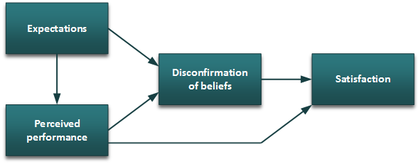
\includegraphics[width=0.95\textwidth]{img/exp.png}
	\caption{Model of Expectation confirmation theory}
	\label{}
\end{figure}

\begin{enumerate}
	\item Product, service quality management is very important.
	\item Managing expectation is important
	\item Overall management is important (Law of multiplication)
\end{enumerate}

To be doing CSM is equivalent to "Market oriented business". Then, the core competence should be endorsed.
\[
\text{CS core competence} = Market Orientation
\]

To be market oriented, you need to collect a lot of data, disseminate them, and utilize them.

Therefore overall, one can make CSM index with two Variable
\begin{enumerate}
	\item Consumer satisfaction index
	\item Market oriented index
\end{enumerate}

Theses are key points of Consumer satisfaction marketing, which is crucial.

\section{Environmental Analysis \& Setting Marketing Goal}


As we have already discussed, within our first step of marketing management system there are 3 main substeps.
\begin{itemize}
	\item Environmental \& Situational analysis
	\item Setting marketing goal
	\item Collecting marketing strategies (STP \& Mix)
\end{itemize}

\subsection{Marketing Goal}

\begin{enumerate}
	\item Financial Goal (Quantitative goal)
	\begin{itemize}
		\item Appearance goal (sales \& market share)
		\begin{itemize}
			\item \texttt{should we build? keep? shrink? shut off(demarketing)?}
			\item type that pushes Growth goal
		\end{itemize}
		\item Net Profit goal (business profit)
		\begin{itemize}
			\item Reduce first cost?
			\item Increase price?
		\end{itemize}
	\end{itemize}
	\item Market Goal (more customer - oriented goal than previous one) (Quality goal)
	\begin{itemize}
		\item Increase Customer satisfaction
		\item Increase brand value
		\item Develop new item
	\end{itemize}
\end{enumerate}

Out of all these different goals, decideing what is necessary is dependent entirely on the situation of the business. Yet, one of the most frequent marketing goal is \textbf{Financial Goal}, and especially \textbf{Growth goal}. Growth goal can be differentiated into 4 areas, give by the chart.

\begin{tabular}{ |c|c|c| }
	\hline
  	& Existing Market & New market \\ [2ex]
	\hline
	Existing Product & penetrate market & Develop market \\ [2ex]
	\hline
	New Product & Develop new product & Diversification \\ [2ex]
	\hline
\end{tabular}

\subsection{Marketing Environment}
If I were to do a business, you can consider the following two cases:
\begin{enumerate}
	\item Market is really good, but I'm really bad.
	\item I am really good, but market is really bad.
\end{enumerate}

Which senario is better? If you think 1st one is better, you are \textbf{Industrial Structuralist}.
According to Porter, there are 5 forces that will effect your business.
\begin{enumerate}
	\item Threat of New entrants
	\item Threat of Substitutes
	\item Power of customers
	\item Power of suppliers
	\item Competitive rivalry
\end{enumerate}

\begin{figure}[H]
	\centering
	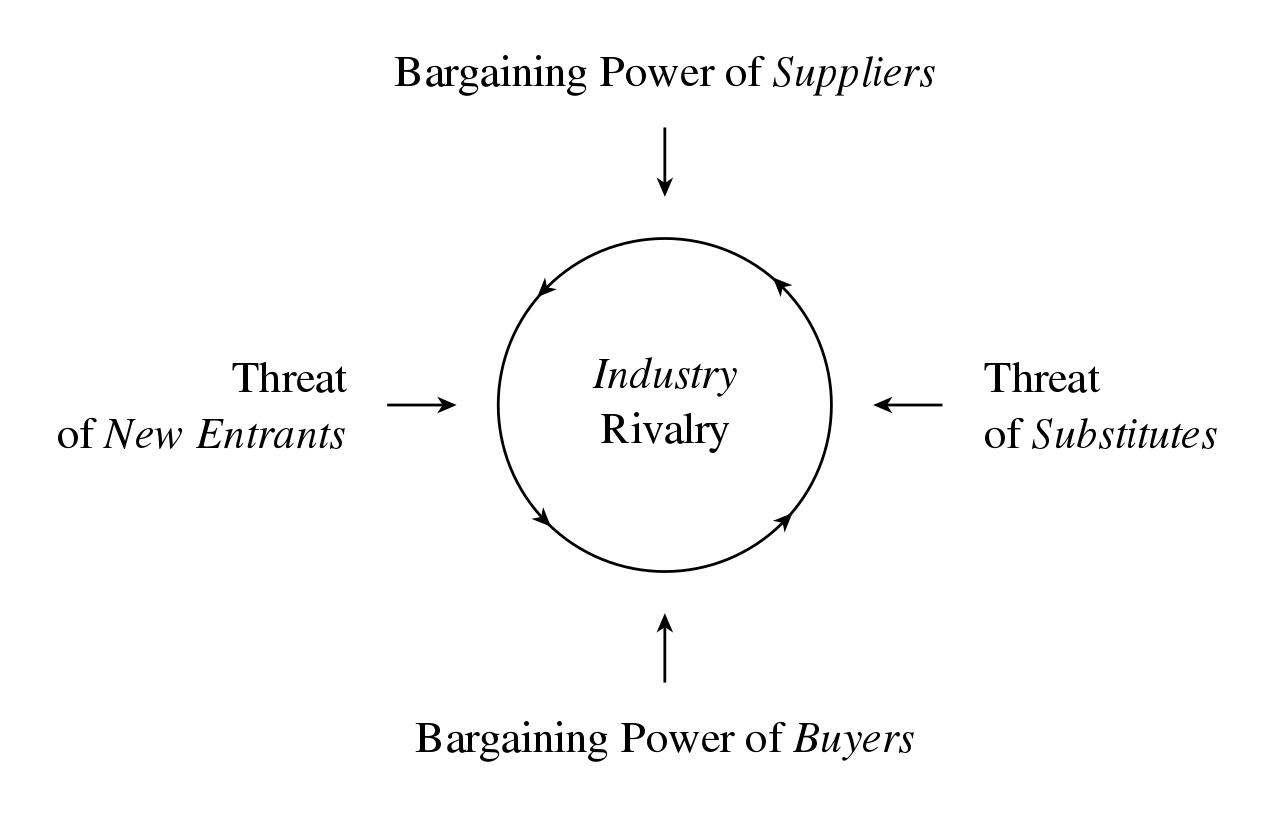
\includegraphics[width=0.95\textwidth]{img/porter5.png}
	\caption{Porter's Five Forces}
	\label{}
\end{figure}

In industrial structure view, you have your environment considered as an outside.
\subsubsection{Outside Environment}
\begin{enumerate}
	\item Macro Environment
	\begin{itemize}
		\item Economy
		\item Tech
		\item Socio - culture
		\item Politics
		\item Law
	\end{itemize}
	\item Micro Environment
	\begin{itemize}
		\item Supply
		\item Demand
		\item Competition
		\item Customer
		\item Business relation
	\end{itemize}
\end{enumerate}

Also you can stand in the position that how well you do in the market is more impactful than your environment. This is called \tb{Resource-Based View} . In this view, you can consider your environment as Inside view.
\subsubsection{Inside Environment}
\tb{Core competence}
\begin{enumerate}
	\item Condition of Core competence: (source of continual competition  frontier -position )
	\begin{itemize}
		\item Needs to be better than competitors
		\item Needs to be difficult to follow.
		\item Needs to be not - purchasable.
		\item Can be implemented to a lot of different businesses
	\end{itemize}
	\item Types of Core competence:
	\begin{itemize}
		\item Form : production line, distribution line, etc...
		\item Formless : Brand, data, formulas, etc...
	\end{itemize}

\end{enumerate}

\tb{Inside situation}

\begin{enumerate}
	\item Business Successfulness
	\begin{itemize}
		\item Financial result (profit, cash flow, debt rate ...)
		\item Market result (market share, customer's evaluation, brand power)
	\end{itemize}
	\item Distribution of usable resources
	\item Prior strategy
\end{enumerate}

Now, when do we really do our environment analysis? Assume that Market goal was made in the spring, and evaluation is ought to be done at winter. What is the most appropriate time for Environmental analysis? \ra \tb{Always}. We collect and watch the data every time, so it can be used anytime.

\smallskip

What is important about theses analysis is the relative change rate. It is almost always about how stuff "change", not how stuff "is".


\subsection{SWAT Analysis}

Factors that engage with your business can be classified into 4 different parts

\smallskip

\begin{tabular}{|c|c|c|}
	\hline
	 & Positive Factor & Negative Factor \\ [2ex]
	 \hline
	 Inside Env & \tb{S}trength & \tb{W}eakness \\[2ex]
	 \hline
	 Outside Env & \tb{O}pportunity & \tb{T}hreat \\ [2ex]
	 \hline

\end{tabular}

\smallskip

Things to Consider about SWAT analysis:

\begin{enumerate}
	\item Collect, collect, collect DATA!
	\item Don't just list and stop, think about their importance.
	\item Make their CROSSSECTION
\end{enumerate}

\begin{figure}[H]
	\centering
	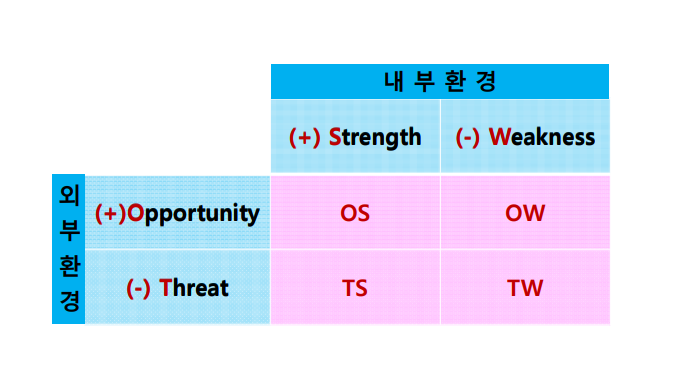
\includegraphics[width=0.95\textwidth]{img/crosssection.png}
	\caption{Crossection of SWOT analysis}
	\label{}
\end{figure}

For example, OW represents how you would manage the opportunity despite your weakness.

We talked about different types of Growth goal. Now it is time to think about more fundamental type of question: Will we grow this business at all? To answer this, we do a portfolio analysis.

\subsection{Product Portfolio Analysis Model}

\subsubsection{Basic Model}
Basic model of portfolio analysis consists of two axis, both of which representing some kind of measure of performance that describes the business.

\begin{figure}[H]
	\centering
	\def\svgwidth{\columnwidth}
	\import{./figures/}{basicmodel.pdf_tex}
	\caption{Basic Model}
	\label{fig:basicmodel}
\end{figure}

\subsubsection{BCG}


The Purpose of BCG model: Set the balance of Cash Flow.
\begin{figure}[H]
	\centering
	\def\svgwidth{\columnwidth}
	\import{./figures/}{BCG.pdf_tex}
	\caption{BCG model}
	\label{fig:BCG Model}
\end{figure}

Problem of BCG Model

\begin{itemize}
  \item Way too simple x, y cord.
  \item Vague definition of market.
  \item Vague borderline of MGR, H/L
  \item Considers only present state.
  \item Can be too drastic.
  \item Don't consider any synergic possibilities.
\end{itemize}

% 1) X as "Position of competition" Y as "Attractiveness of Business"
%
% 2) Define market within realm of SUB
%
% 3) High - Medium - Low

%9월 11일


\section{Marketing Research}

\subsection{Marketing research Steps}

1. Analyzing situation step
\begin{itemize}
	\item Changes in Inside, outside Environments
	\item Strength, weakness of our, opponent companies
	\item catching opportunities/analyzing market character
	\item analyzing consumers
\end{itemize}

2. Collecting strategies step
\begin{itemize}
	\item Researching consumer's recognition
	\item Marketing test (concept, elasticity of price, prediction of demand, effectiveness of ad)
\end{itemize}

3. Execute strategies step
\begin{itemize}
	\item Ad tracking (ad acceptance rate, recognition rate, product recognition rate ...)
	\item New product tracking (recognition, preference ... )
\end{itemize}

4. Evaluate step
market share, mind share, brand equity, satisfaction etc...



How do we get the data?
\begin{enumerate}
	\item Search for it (online, researches...)
	\item Make them!
	\item Buy them! (or let others make them)
\end{enumerate}

\subsection{Marketing Research Process}

\begin{enumerate}
	\item Decide whether we need to research
	\item Specify why we need to research (specifically research for what?)
	\item Types of research construction
	\item Data Source (Do we make them? search for it? etc..)
	\item How do we collect our data?
	\item Extract samples and collect Data (what is our sample group? how? how many?)
	\item Analysis of our data (coding, correlational analysis, causal analysis...)
	\item Organize the result.
\end{enumerate}

\subsubsection{Type of research construction}
\begin{enumerate}
	\item Exploratory research
	\begin{itemize}
		\item "Why do we lack net profit?"
		\item "would single family's consuming mind different?"
	\end{itemize}
	\item Descriptive research (much more enumerative and analytical, more to correlational study)
	\begin{itemize}
		\item "Is the reason of lack of net profit differ by different areas?"
		\item "Is the single family consumer sentiment differ by different age?"
	\end{itemize}
	\item Causal research (not much correlational, more causality research)
	\begin{itemize}
		\item "Is price discount better than quantity discount?"
		\item "Is minimalization better than advancing?"
	\end{itemize}
%Class 4_: 오후 3시 50분 ~ 4시 20분 사이 (탐색, 기술, 인과 조사 설명들...)

\end{enumerate}
\subsubsection{Data source}
\begin{enumerate}
	\item Secondary Data
	\begin{itemize}
		\item Inside data (Business related data..)
		\item Outside data (통계청, 국책연구소, 민간경제연구소, 상공회의소 등...)
	\end{itemize}
	\item Primary data
	\begin{itemize}
		\item survey, test (Field, Laboratory, fMRI)
		\item Observation and interview
	\end{itemize}
	\item New raw Data
	\begin{itemize}
		\item Purchase Data
		\item clickstream Data
		\item UCC, SNS Data
		\item Big data (3V's: volume, variety, velocity)
	\end{itemize}
\end{enumerate}

\subsubsection{Example: Coke or Pepsi?}

Pepsi Challenge

"New coke" blunder

Despite all the research, why did so many people hate New coke?

"are you sure that taste only comes with tongue?"

By doing fMRI study of brain, one can find out that while blind testing, VMPFC of brain was triggered, while drinking coke, DLPFC and Hippocampus was triggered.

\subsubsection{Method of collecting Data (Survey)}

\begin{enumerate}
	\item Collecting Method
	\begin{itemize}
		\item face-to-face/or not
		\item mail, phone
		\item online
		\item mobile
	\end{itemize}
	\item Sampling
	\begin{itemize}
		\item sampling frame (list of things you draw a sample from)
		\item method of sampling (random sampling/easy sampling)
		\item sampling size
	\end{itemize}
\end{enumerate}

\subsubsection{Research Analysis}

\begin{enumerate}
	\item Statistical Analysis
	\begin{itemize}
		\item univariable analysis
		\item multivariable analysis
		\item non - parametric analysis
	\end{itemize}
	\item Analyzing meaning
	\begin{itemize}
		\item correlational
		\item Causal
	\end{itemize}
\end{enumerate}

\section{Consumer Behavior Analysis}
\subsection{Frame of Consumer behavior analysis}
1. Understanding consumer's Perspective
\begin{itemize}
	\item who? (who is our customer?)
	\item what would they want?
	\item How would they react? (to this product?)
	\item why?
\end{itemize}

For consumer, there are 5 steps that takes place per every purchasement.
2. 5 Decision making steps
\begin{enumerate}
	\item facing the problem
	\item searching for information
	\item look for alternative
	\item Buying the product
	\item Action after purchase (usage and feedback)
\end{enumerate}

Who would face the problem? Not necessarily the one who uses. They can be his/her parents, related people, friends, ... etc..

In similar fashion, who would search for alternative? Who would actually purchase? Above steps can be done by all separate people.
The 2. can be questioned by 1. therefore 20 questions can arise in total. However, the 1. can be much more descriptive.

Personal traits can be influential to individual decision steps. This can be,
\begin{itemize}
	\item Memory
	\item attitude.
	\item etc...
\end{itemize}

Moreover environmental traits can be also influential. This can be:
\begin{itemize}
	\item Demographical statistic
	\item Economic situation
	\item Socio - cultural
	\item Technological env.
	\item Law - related env.
\end{itemize}

Therefore theses factors play great role on understanding consumer's behaviors.

\subsection{General Characteristics of Consumer Behaviors}

Every consumer is human, therefore behaves in very "generalizable" way. It is natural to think that people behave in calculative, rational way. But this turned out to be very wrong.

\begin{enumerate}
	\item Decision making method routinized
	\begin{itemize}
		\item Extensive problem solving (Searching for all possible info)
		\item Limited problem solving (not thinking carefully)
		\item Routinized behavior
	\end{itemize}
	\item Behaviors within relationships(Between other objective beings)
	\begin{itemize}
		\item Reference group influence (e.g. by pressure, I'm now fine with alcohol)
		\item Trickle down Effect
		There are differences between social hierarchy within behavior of consumers. So called "lower class" tends to follow "higher class"
		\item Social modeling (People tends to follow other people in general. especially who they admire)
		Why is it that, despite not believing the model is only working for "money", the influence is still there. This works for other examples not bounded by human models.
		\begin{figure}[H]
	\centering
	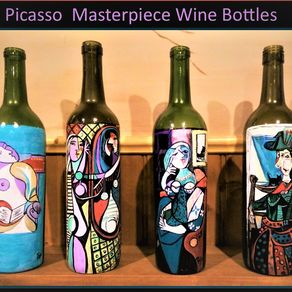
\includegraphics[width=0.95\textwidth]{img/picawine.png}
	\caption{Wine bottle with image of Picasso sells dramatically}
	\label{}
\end{figure}

	\end{itemize}
	\item Expected Irrationality (We are very irrational indeed, but we are irrational in very rational way. Therefore, pre-calculatable)
	\begin{itemize}
		\item Heuristics and biases
		\item  Emotional decisions
		\item Non conscious behaviors (Done without conscious)
	\end{itemize}
\end{enumerate}

Theses behaviors can be (in a way) predicted by marketers, making marketing process much efficient.
How many of us make un-rational decisions? about 80\%(says our professor).

\begin{figure}[H]
	\centering
	\def\svgwidth{\columnwidth}
	\import{./figures/}{consumerMotivation.pdf_tex}
	\caption{What drives consumer Motivation?}
	\label{fig:consumerMotivation}
\end{figure}

\subsubsection{Consumer Behavior's Megatrend (keyword)}
\begin{itemize}
	\item Consumer rights
	\item Produmer (producer and both consumer)
	\item Life's quality (well being, health, prestige, small luxury)
	\item Green Friendly (ethical, green, shared consumption)
	\item High-Tech (Mobile, AI, IoT, VR, Robot)
	\item Decision disorder (info overload, decision curator)
\end{itemize}

\section{Segmentation and Targeting}

Now we collect strategies. We will start with STP. In this section, we will look at S and T.

\subsection{Segmentation}

Definition: splitting the market into few 'segments', to be considered later.


But do we really need market segmentation?

\subsubsection{Necessity of Market Segmentation}

First, the customers are very different. \ra You can be very precise to customer's needs.

Also, the company has very limited resources. \ra You can choose and focus on one point.

And finally, there are just too much competition.
Segmenting makes different opportunities stand out
very easily.
Plus, you can also act very quickly to changes.

\begin{figure}[H]
	\centering
	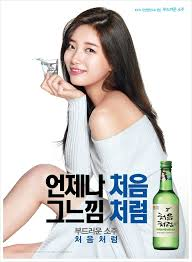
\includegraphics[width=0.95\textwidth]{img/soju.png}
	\caption{Target market : Easily enjoying liquor, for age 20 \~30, woman, lives in cities.}
	\label{soju}
\end{figure}


\subsubsection{Standards for Market segmentation}

\begin{itemize}
	\item Geological variable \ra weather, pop density, areas
	\item Demographic variable \ra age, gender, income level, educational, job
	\item Psychological variable \ra Values, personality traits, motivation, lifestyle
	\item Behavioral variable \ra Pursuit of convenience , amount of usage, preferences, bargaining
\end{itemize}

\textbf{Geological, Populational-statistical Variable (i.e. Demographic variable)}

\begin{itemize}
	\item Sometimes define the demand for entire category!! (weather, population, age, gender, income level)
	\item Creates \textbf{subculture} (Generation wise, jobwise, area wise culture)
	\item Customer Porfile elements \ra "accessibility" (who are they? How do we(company) approach them?)
\end{itemize}

\begin{tcolorbox}
	\textbf{Example}: Cookies (HaeTae and Lotte)
	\begin{center}
		Do cookies really need market segmentation?
	\end{center}
	You can make an argument that everyone likes cookies. Almost everyone consumes cookies. Yet, there seemed to be \textbf{geological difference} between areas. Why is that? Even though heavy consumers are children, it seemed like area's conflict seemed to be engaged: Therefore focus on the \textbf{distributor}. Thing are getting better nowdays. link:
	http://www.donga.com/news/article/all/20030826/7976875/1

\end{tcolorbox}

\textbf{Psychological Variable}
\begin{itemize}
	\item Effects almost every aspect of consumer's behavior (values, personality traits, lifestyle etc...)
	\item One of the Customer's profile's elements : \ra Appealing methods (How do we invoke consumer's motivation to buy?)
\end{itemize}
\textbf{Question: How do you segment market by personal values?}

\sk

{\large \textit{LOV Segmentation}}

\sk

1. Main Value measurement
\begin{itemize}
	\item  Rokeach survay (36 value items)
	\item List of value (LOV) (9 value items)

\end{itemize}

2. Rounding off by main values \ra \textbf{Factor analysis}

3.Making Segments \ra \textbf{Clustering analysis}

\begin{tcolorbox}
	Question: How do you exactly do factor analysis?
	% 자긍, 자아실현, 성취 존경 : factor 1
	% 존겨으 재미, 흥 : factor 2
	% 안저으 소속, 대인관계: factor 3
\end{tcolorbox}

After factor analysis, you make clustering by looking at the data.

% \begin{figure}[H]
% 	\centering
% 	\def\svgwidth{\columnwidth}
% 	\import{./figures/}{clustering.pdf_tex}
% 	\caption{Clustering}
% 	\label{fig:clustering}
% \end{figure}

\sk

\textbf{Behavioral Variable}

\begin{itemize}
	\item Craving product benefit
	\item Heavy user/ Light user
	\item Reaction Step: (recognition\ra knowledge \ra preferable \ra buying experience \ra recursive purchase)
	Example :
	if everyone likes it and nobody buys it, there must be purchase obstacle.

	if nobody knows it, must let them know first.

	if everyone know it but nobody likes it, change their attitude.

	etc etc...
	\item Price sensitivity
	\item Usage situation: ( Where do people use our product?)
	\item Accepting innovative product (Would they buy beta version?)

\end{itemize}

{\large In what variable do we use to segment market?}

* \textbf{Let's think...}
\begin{enumerate}
	\item Using any standard, market does get segmented. (Now is it just matter of your choice?)
	\item You simply can't use all the standards, because it isn't profitable and way too complicated. \ra \textbf{use right amount}
	\item Thus you need \textbf{Efficient market segmenntation}
\end{enumerate}

\subsection{Effective Market Segmentation}
{\large Effectiveness:::}
\begin{enumerate}
	\item Measurable %What??
	\item Accessible
	\item Substantial (Segmented by 99 : 1 is just meaningless. There has to be meaningfulness)
	\item Differentiable by segments (if strategies among segments are equal, it is meaningless)
\end{enumerate}

\ra Yet, \textbf{per variable, Effectiveness is different.} %어떤 변수는 이런 쪽에서 효율이 좋지만 이런 쪽에선 안좋음

\subsubsection{How do you deal with that? Wedel \& Kamakura's}
\begin{center}
	\begin{tabular}{m{12em}|m{12em}|m{12em}|}
		\hline
		& General character variable & Prdouct related variable \\ [2ex]
		\hline
		Observable & Demographical & Usage, Use situ, Royalty \\ [2ex]
		\hline
		Non Observable & Per Trait, LOV, lifestyle & Preference, recognition of product \\ [2ex]
		\hline

\end{tabular}
\end{center}

\begin{tabular}{|c|c|c|c|c|}
	\hline
	 & G/O & G/NO & P/O & P/NO \\

\end{tabular}

{\large Then what??}

\begin{itemize}
	\item Use Multiple Variable
	\item Actionable Variable
	\item use high - Accesiable variable to make profile.
\end{itemize}

\subsection{Steps for Market Segmentation}

\begin{enumerate}
	\item Collect Data
	\item Measure variable by marketing search
	\item Segment by actionable variable
	\item Make Profile for each segmented market.
\end{enumerate}


	Toothpaste Market:

\begin{tcolorbox}
	Product benifit can be very different


\end{tcolorbox}

\subsection{Time variant Segmentation}

How do you segment markets real- time? Well, after fully knowing the method, you still don't know what will come out as an result, nor what is really efficient.
Knowing certain stuff beforehand can be described as \textbf{a priori segmentation}, other is \textbf{a posterior segmentation}
\begin{figure}[H]
	\centering
	\def\svgwidth{\columnwidth}
	\import{./figures/}{mseapr.pdf_tex}
	\caption{Different segment}
	\label{fig:mseapr}
\end{figure}
For example LOV, you knew how you choose the segmenting method, but you didn't know the result. The result of 4 factor can be considered as a posterior.


\section{Targeting}

Ok. you've segmented the market. (that was hard) Now you have to choose what part of segemtn you are going to be engaging in.

\subsection{Standards for Target segment's Decision}

\tb{1. Segment's attractiveness}
\begin{itemize}
	\item Outside conditions (market size, potential, growth rate, product's life cycle, seasonal)
	\item Structural condition (competition difficulty, threat of alternatives, power of buyer/producer, Wall of entrance(진입장벽))
	\item Environmental condition (Economy, society, ...)
\end{itemize}

\sk

\tb{2. Relative competitive position within the segment}

How well will your company do when you enter the segment? To answer this, you need to know how much strength you have (competence) against others, for these following example categories:
\begin{itemize}
	\item differentiated strength?
	\item Price strength?
	\item Operative strength?
\end{itemize}

{\large The way "competition" is defined can be varied by level}


\begin{itemize}
	\item By brand (e.g: Digital Camera 1 vs Digital Camera 2)
	\item Form of product {e.g: Digital Camera vs DSLR vs Mirrorless}
	\item Fundamental convenience (e.g: D.c vs Phone)
\end{itemize}

\textit{Example: Asking frontier brand's most fearful competitor}

\begin{tcolorbox}
	\begin{itemize}
		\item chamisul \ra samsung TV
		\item Lineage \ra America Drama
		\item sulwhasu \ra Korean medic
		\item Bakcas \ra Starbucks
		\item Nike \ra Nintendo
	\end{itemize}
\end{tcolorbox}

\begin{center}
	{\Large \textbf{Marketing Myopia}}
	\ra look at the market from long distance. ( would above competition make sense?)
	the fundamental values can be provided by much different product. Therefore beware of not - knowing your place or your competitors.
\end{center}

\tb{3. Compatibility}

with...
\begin{itemize}
	\item company resources
	\item company's mission \& culture
	\item existing market, existing marketing mix.
\end{itemize}

Now all these standards can be calculated and weighted - summed, so one can decide which market segments to enter.

Then, Target market can be treated
\begin{itemize}
	\item as differentiated into one or more segments.
	\item or treated as same or different
\end{itemize}

\subsection{Treating Segments differently: How much?}
The more you differentiate your treatment to targeted market, the more you'll earn, but also more you'll investigate. Therefore one has to find the right balance.


\section{Postitioning}
Definition: finding position inside consumer's \textbf{mind}

\begin{itemize}
	\item competitive differentiation consumer perceive
	\item problem of competitive structure's overall harmonizing marketing mix.
	\item Not reality, just perception
	\item Can define direct competitors
	\item Can grasp market opportunities
\end{itemize}
\subsection{Positioning Map}

\begin{figure}[H]
	\centering
	\def\svgwidth{\columnwidth}
	\import{./figures/}{pmap.pdf_tex}
	\caption{Structure of positioning map}
	\label{fig:pmap}
\end{figure}
\subsubsection{Making of positioning map}
\begin{enumerate}
	\item Multi Attribute Model (MAM)
	\ra what constitutes a product is used as axis. (and how good they are per product of different companies)
	\item Multi Dimensional Scaling (MDS)
	\ra Asking consumers for unknown axis, and trying to search for axis.
\end{enumerate}

1. MAM
\begin{itemize}
	\item grasp main character of products.
	\item Per product, find the values for characters.
	\item Factor Analysis
	\begin{itemize}
		\item figuring out the underlying dimensions
		\item find the scale value per theses basis dimension.
	\end{itemize}
	\item  Make positioning map.
\end{itemize}

2. MDS
\begin{tcolorbox}
	"Making positioning map under recognition of consumer's similarity"

\end{tcolorbox}
Ask customer's their measure of similarity of different products.

\begin{figure}[H]
	\centering
	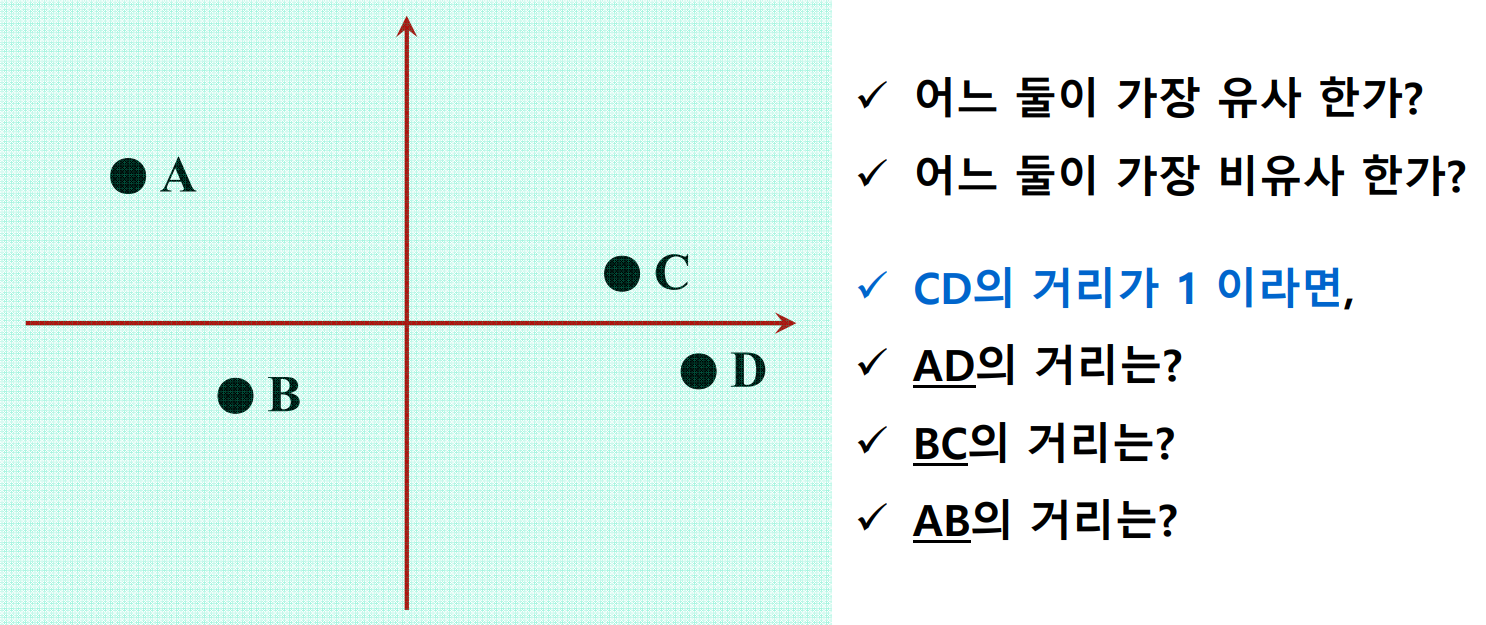
\includegraphics[width=0.95\textwidth]{img/mds.png}
	\caption{}
	\label{}
\end{figure}

\subsection{Positioning Strategy}
Here we will talk about:
\begin{enumerate}
	\item Overall Quality - Price positioning
	\item Specific POD(point of difference) positioning
	\item condition of Efficient positioning
\end{enumerate}
\subsection{Overall Quality - Price positioning}
\begin{figure}[H]
	\centering
	\def\svgwidth{\columnwidth}
	\import{./figures/}{oqpp.pdf_tex}
	\caption{Simple MAM with price, quality axis.}
	\label{fig:oqpp}
\end{figure}



\subsection{Specific POD(point of difference) positioning}
\begin{itemize}
	\item property POD
	\item Service POD
	\item User POD
	\item Usage situation POD
\end{itemize}
{\large Many time, positioning is done with specific property POD}

But sometimes, user specific POD is made.
(풀무원:(환경친화적인 당신은) 이미 풀무원입니다)

\subsection{Efficient POD condition}
\begin{enumerate}
	\item POD's dimension is important
	\item That difference must be perceived meaningfully
\end{enumerate}

\begin{center}
	Meaningful POD vs not! meaningful POD

\end{center}
\begin{enumerate}
	\item Work in existing field,\ra make strategies within known map
	\begin{itemize}
		\item difference within already existing dimension
		\item comparing quality between other competitors ("alignable" difference)
		examples could be (cheaper, bigger, tastes better, stronger, faster etc...)
		\item Property based POD is almost all this case
	\end{itemize}
	\item Change the existing field \ra taking strategies to change the existing map
	\begin{itemize}
		\item Have property that no others have. : (nonalignable difference)
		\item Changes structure of Positioning map by introducing new axis!
	\end{itemize}
\end{enumerate}
\subsubsection{Case 1. Make strategies within known map}
Here, the specific dimension is very important, but the problem is that "challenger's" claim isn't well informed. Specifically,
\begin{itemize}
	\item Most of the difference is ignored (Prototype effect)
	\item Especially qualities that aren't directly noticeable.
\end{itemize}
Then how do we solve this problem? 3 possible approaches :
\begin{itemize}
	\item noticeable Property (Searchable property vs Experienceable property vs trust based property)
	\item Enough difference
	\item Enumerable difference
\end{itemize}

\subsubsection{Case 2.POD engaging New property dimension}
New property must be meaningful one.
But making consumer recognize their importance is not EASY. Then how do we solve this problem?
\begin{itemize}
	\item Density prinicple
	\begin{itemize}
		\item makie perception's density higher. (variants, voice, shelf space)
	\end{itemize}
	\item Synergy principle
	\begin{itemize}
		\item across ads \& over time, linearity within contents
	\end{itemize}
	\item Categorization effect
	\begin{itemize}
		\item Category label (subcategorization) : put category on our product within this market, and label it so that others can perceive it.
	\end{itemize}
\end{itemize}

\subsection{Positioning Step}
\begin{center}
\begin{enumerate}
	\item Analyze  current position (Make positioning map)

	\ra MAM or MDS
	\item Choose goal position
	\item Execute Repositioning strategies
	\item Evaluate transformed position (Make positioning map again!)
\end{enumerate}

\end{center}

\section{Product Life Cycle}
\begin{tcolorbox}
	Product viewed as Life(metaphor)

	Birth \ra growth \ra maturity \ra decline \ra death

\end{tcolorbox}
: {\large to know what stage our product is, to take action accordingly.}

\begin{figure}[H]
	\centering
	\def\svgwidth{\columnwidth}
	\import{./figures/}{plc.pdf_tex}
	\caption{Graph of Product life cycle}
	\label{fig:plc}
\end{figure}

Marketing goal must be very different according to the stage of PLC they are in.
\tb{Example:}


Entering Stage : Create AW \& trial
Growing Stage L Maximize MS
Mature Stage: Max profit \& MS
Decline Stage : Reduce Expenditure

\subsection{Unit of analyzing PLC}
\begin{enumerate}
	\item Product class
	\item Product form
	\item Brand
\end{enumerate}

\begin{center}
	\begin{enumerate}
		\item Hard to predic "which stage" \& "how long"
		\item Self - fulfilling prophecy (: If you decide on which stage you are in, you will be in that stage)
	\end{enumerate}

\end{center}

\section{Product Management \& NPD (new product development)}

\subsection{Product Management Basic}

A. Concept of Product.

\begin{enumerate}
	\item Core Product
	\item Actual Product
	\item Augmented Product
\end{enumerate}

\begin{figure}[H]
	\centering
	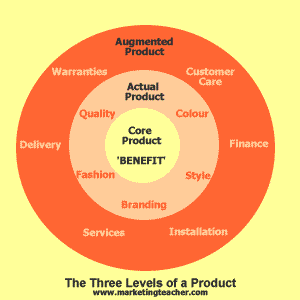
\includegraphics[width=0.95\textwidth]{img/caa.png}
	\caption{Examples of Core products (From www.marketingteacher.com)}
	\label{}
\end{figure}
If we were to differentiate from the enemy company, there are these 3 options to be made.

B. Product Classification

\begin{enumerate}
	\item Industrial goods vs Consumer goods
	\item  Durable goods vs non-durable goods vs services %(at 5 min, 9/23)
	\item Convenience goods vs Shopping goods vs Special goods
	\item  Exploratory based vs Experience based vs Trust based
\end{enumerate}

C. Product mix

\begin{itemize}
	\item Width of Product mix \ra number of product line within company
	\item Product line \ra category of related product
	\item Length of Product line L \ra number of Brands per one product line
	\item Depth of Product line. \ra number of items in one brand.
\end{itemize}


\textbf{Example :} P\&G product Mix.



\begin{tabular}{c|c|c|c|c|c}
	\hline
	Baby Care & Fabric care & Oral care & Skin care & hair care & home care \\
	\hline
	Luvs & Tide Crest & Ivory & Head\&Shol & Febreze \\
	Pampers & Cheer & oral- B & SK-II & Pantene & Cascade \\
	 & Bounce & Scope & Gillette & Old spice & Dawn \\
	 & Downy & Fixodent & Olay \\

\end{tabular}

D. Level of New Product.

By the quality of improvement by new product, we can classify the new product's level

\begin{enumerate}
	\item Simple Renewal \\
	this can be caused by...
	\begin{itemize}
		\item Increased price
		\item simply renew the feeling
		\item etc...
	\end{itemize}
	 \item Product Variants / Improvement (Just improving a bit)
	 \item Product line-up (What do you mean by lineup?) \\
	 \ra Constituted by product quality \& price. (i.e. New item is much better and expensive. This is different by case 1)
	 \item New Product - New line /Category (\textbf{new} is to be taken relative to myself.) \\
	 \begin{itemize}
	 	\item Continuous innovation
		\item Dynamically continuous innovation.
		\item Discontinuous innovation
	 \end{itemize}

\end{enumerate}

\subsection{Main Content within Product management}
\begin{itemize}
	\item Managing individual products.  (renewal, morphism, improvement)
	\item Decisions within product line (i.e. portfolio management with multiple items) \\
	So why do we need  Product length/depth?
	\begin{itemize}
		\item Consumer's need is very different.
		\item People crave for diversity. (we never consume one food)
		\item Price sensitivity differ.
		\item Inhibit other company's competitive entry.
		\item Positioning (Making Subcategory (This is necessary for "density" condition.))
	\end{itemize}

	But what are some considerations?

	\begin{itemize}
		\item Increase of Cost. (making diverse product inevitably increases price.)
		\item Distribution's cooperation.
		\item confusion of consumer's recognition
		\item Cannibalization / Synergy
		\item Enough Resources and management capacity
	\end{itemize}

	\item Managing NPD
\end{itemize}

\subsection{Developing New product}
\begin{itemize}
	\item Managing NPD
	\item Market Testing NP
\end{itemize}
\subsubsection{Is making New product actually necessary?}
It is
\begin{enumerate}
	\item Resource of Company's Growth. (i.e. you can't make consumers buy a single thing forever!)
	\item Method of Market's Attack and Defense (as a matter of competition.) \\
	\begin{itemize}
		\item Flanker Brand (As a defense to attacker in a market (they will have cheaper - item attack) , usually make cheaper item to defend)
		\item Fighter Brand (As an attack)
		\item Decoy Brand (as a trap) \\
		\tb{e.g.} : Magazine Economist has 3 options for subscription
		\begin{itemize}
			\item online (59\$)
			\item offline (125 \$) \ra this item is decoy brand
			\item online + offline (125\$)
		\end{itemize}
	\end{itemize}
	\item At mature market, make alternative need by making new product.
	\item As a leader of industry, need to keep the reputation.
\end{enumerate}
And importantly,

\textbf{Pioneer Advantage}

\subsection{Why would some New product fail?}
%1 h 5min
\begin{itemize}
	\item Null of differentiated convenience
	\item Change of consumer's utility
	\item Targeting/ positioning problem
	\item Timing of release
	\item Error within demand estimate
	\item etc etc...
\end{itemize}

\subsection{Management system for developing new product}

\begin{figure}[H]
	\centering
	\def\svgwidth{\columnwidth}
	\import{./figures/}{npdman.pdf_tex}
	\caption{New Product Development Managing System}
	\label{fig:npdman}
\end{figure}

\subsubsection{Deciding New Product idea}

There are a lot of different origin of ideas and many methodologies.

From there, we extract the ideas, which we then decide what idea we will choose.

It is important to produce many ideas (Because this is very cheep!)

\ra \textbf{Thus, Diversify origin and Methodology}.

Where do we get the idea? (Origin of ideas)

\begin{itemize}
	\item Customers
	\item Competitor
	\item Inside community \\
	\begin{itemize}
		\item R\&D
		\item Idea Team
		\item Idea institution
	\end{itemize}
	\item Distributor, Selling member
	\item Socialnet Data
\end{itemize}
\nii
How do we make the data? (Methodology)
\begin{itemize}
	\item Brainstorming
	\item FGI
	\item Town watching
	\item Trend analysis
	\item Attribute Listing
	\item etc etc...
\end{itemize}

\begin{center}{
	\large Make the chosen idea more specific.

	\sk

	\ra Product Concept
	}

\end{center}


\subsubsection{Idea Into Product concept}
Definition:
\begin{tcolorbox}
	Product idea \tb{described as manner of consumer's perspective}, such as
	product's shape, character, utility, convenience, price etc...

\end{tcolorbox}

\begin{itemize}
	\item What property and character? (Product attributes)
	\item Gives what? (consumer Benefit Proposition)
	\item Usage situation
	\item For whom? (Target consumer)
	\item Price and distribution? (Marketing mix)
	\item etc ..
\end{itemize}

\subsubsection{Concept Test, Design Test}

As we make concept and design, we need to test them simultaneously.]\

\sk

Conjoint analysis : make a lot of profile \\
\ra choose the feasible profile and ask them for which is most reasonable.


Purchase intention

Also, make standard evaluation chart beforehand.

Test standard:
\begin{itemize}
	\item Technological feasibility
	\item Trade feasibility
\end{itemize}

At NPD's beginning Step, everybody's participation is important!


 * Potential net profit model.

\begin{enumerate}
	\item Transforming "purchase intension" / preference chart
	\item Making selling formation model (46 min 판매형성 모형)
	\[
	 P = A_w A_v \sum B_c
	\]
\end{enumerate}
\begin{enumerate}
	\item lab test
	\item Pro test
	\item Customer test (Conjoint analysis)
\end{enumerate}

\subsubsection{Test market}

\begin{enumerate}
	\item Purpose : \begin{itemize}
		\item much precise net profit estimate
		\item getting diagnostic information
	\end{itemize}
	\item Types : \begin{itemize}
		\item National - scale market reenactment
		\item Experimental method (mini test market )
	\end{itemize}
	\item Weakness \begin{itemize}
		\item High price
		\item Competitor's recognition and disturbances
		\item Delay of release
	\end{itemize}
\end{enumerate}

\subsubsection{Pre - test market}

\begin{enumerate}
	\item Purpose, \begin{itemize}
		\item Appropriate prediction made (75\% and above)
		\item Reasonably accurate tests
		\item Not much time consuming
		\item Relatively low price
	\end{itemize}
	\item Typs :
	\begin{itemize}
		\item Non- durable model (e.g. ASSESSOR)
		\item Durable model (e.g. Information Acceleration)
	\end{itemize}

\end{enumerate}


\end{document}
